% Created 2023-06-23 Fri 07:33
\documentclass[9pt, b5paper]{article}
\usepackage{xeCJK}
\usepackage[T1]{fontenc}
\usepackage{bera}
\usepackage[scaled]{beraserif}
\usepackage[scaled]{berasans}
\usepackage[scaled]{beramono}
\usepackage[cache=false]{minted}
\usepackage{xltxtra}
\usepackage{graphicx}
\usepackage{xcolor}
\usepackage{multirow}
\usepackage{multicol}
\usepackage{float}
\usepackage{textcomp}
\usepackage{algorithm}
\usepackage{algorithmic}
\usepackage{latexsym}
\usepackage{natbib}
\usepackage{geometry}
\geometry{left=1.2cm,right=1.2cm,top=1.5cm,bottom=1.2cm}
\usepackage[xetex,colorlinks=true,CJKbookmarks=true,linkcolor=blue,urlcolor=blue,menucolor=blue]{hyperref}
\newminted{common-lisp}{fontsize=\footnotesize} 
\author{deepwaterooo}
\date{\today}
\title{ET 框架学习笔记--自己需要这样一个总结文档来帮助总结与急速重构自己的游戏}
\hypersetup{
  pdfkeywords={},
  pdfsubject={},
  pdfcreator={Emacs 28.2 (Org mode 8.2.7c)}}
\begin{document}

\maketitle
\tableofcontents


\section{客户端场景组件:客户端大致的起始过程}
\label{sec-1}
\subsection{Entry.cs: 指定的起始类,会触发三类回调,公用组件类的加载,和其它}
\label{sec-1-1}
\begin{minted}[fontsize=\scriptsize,linenos=false]{csharp}
public static class Entry {
    public static void Init() {
    }
    public static void Start() {
        StartAsync().Coroutine();
    }
    // 【各种应用程序,第三方库等的初始化 】
    private static async ETTask StartAsync() {
        WinPeriod.Init();

        MongoHelper.Init();
        ProtobufHelper.Init();

        Game.AddSingleton<NetServices>();
        Game.AddSingleton<Root>();
        await Game.AddSingleton<ConfigComponent>().LoadAsync();

        // 不知道:加这三个是在做什么?它没有起有意义的名字,但总之,它是事件,会触发相应的回调
        await EventSystem.Instance.PublishAsync(Root.Instance.Scene, new EventType.EntryEvent1());
        await EventSystem.Instance.PublishAsync(Root.Instance.Scene, new EventType.EntryEvent2());
        await EventSystem.Instance.PublishAsync(Root.Instance.Scene, new EventType.EntryEvent3());
    }
}
\end{minted}
\subsection{EntryEvent1\_InitShare: 第一类,,公用组件类的加载,公用的几大组件}
\label{sec-1-2}
\begin{minted}[fontsize=\scriptsize,linenos=false]{csharp}
// 公用的相关组件的初始化:
[Event(SceneType.Process)]
public class EntryEvent1_InitShare: AEvent<EventType.EntryEvent1> {
    protected override async ETTask Run(Scene scene, EventType.EntryEvent1 args) {
        Root.Instance.Scene.AddComponent<NetThreadComponent>();
        Root.Instance.Scene.AddComponent<OpcodeTypeComponent>();
        Root.Instance.Scene.AddComponent<MessageDispatcherComponent>();
        Root.Instance.Scene.AddComponent<NumericWatcherComponent>();
        Root.Instance.Scene.AddComponent<AIDispatcherComponent>();
        Root.Instance.Scene.AddComponent<ClientSceneManagerComponent>();
        await ETTask.CompletedTask;
    }
}
\end{minted}
\subsubsection{CurrentScenesComponent: 可以用来管理多个客户端场景,比如大世界会加载多块场景(是说,大地图可以分10 块 8 块小地图吗? )}
\label{sec-1-2-1}
\begin{minted}[fontsize=\scriptsize,linenos=false]{csharp}
// 可以用来管理多个客户端场景,比如大世界会加载多块场景(意思是说,大地图可以分10 块 8 块小地图吗? )
[ComponentOf(typeof(Scene))]
public class CurrentScenesComponent: Entity, IAwake {
    public Scene Scene { get; set; }
}
\end{minted}
\subsubsection{CurrentScenesComponentSystem: CurrentScene() 方法,返回当前场景}
\label{sec-1-2-2}
\begin{minted}[fontsize=\scriptsize,linenos=false]{csharp}
public static class CurrentScenesComponentSystem {
    public static Scene CurrentScene(this Scene clientScene) {
        return clientScene.GetComponent<CurrentScenesComponent>()?.Scene;
    }
}
\end{minted}
\subsubsection{ObjectWait: 也有生成系}
\label{sec-1-2-3}
\begin{minted}[fontsize=\scriptsize,linenos=false]{csharp}
[ComponentOf]
public class ObjectWait: Entity, IAwake, IDestroy {
    public Dictionary<Type, object> tcss = new Dictionary<Type, object>();
}
\end{minted}
\subsubsection{PlayerComponent:}
\label{sec-1-2-4}
\begin{minted}[fontsize=\scriptsize,linenos=false]{csharp}
[ComponentOf(typeof(Scene))]
public class PlayerComponent: Entity, IAwake {
    public long MyId { get; set; }
}
\end{minted}
\subsubsection{PlayerComponentSystem: 生成系,到处都要用它}
\label{sec-1-2-5}
\begin{minted}[fontsize=\scriptsize,linenos=false]{csharp}
[FriendOf(typeof(PlayerComponent))]
public static class PlayerComponentSystem {
    public static void Add(this PlayerComponent self, Player player) {
        self.idPlayers.Add(player.Id, player);
    }
    public static Player Get(this PlayerComponent self, long id) {
        self.idPlayers.TryGetValue(id, out Player gamer);
        return gamer;
    }
    public static void Remove(this PlayerComponent self, long id) {
        self.idPlayers.Remove(id);
    }
    public static Player[] GetAll(this PlayerComponent self) {
        return self.idPlayers.Values.ToArray();
    }
}
\end{minted}
\subsection{AfterCreateCurrentScene\_AddComponent:【UIComponent】【ResourcesLoaderComponent】}
\label{sec-1-3}
\begin{minted}[fontsize=\scriptsize,linenos=false]{csharp}
[Event(SceneType.Current)]
public class AfterCreateCurrentScene_AddComponent: AEvent<EventType.AfterCreateCurrentScene> {
    protected override async ETTask Run(Scene scene, EventType.AfterCreateCurrentScene args) {
        scene.AddComponent<UIComponent>();
        scene.AddComponent<ResourcesLoaderComponent>();
        await ETTask.CompletedTask;
    }
}
\end{minted}
\subsubsection{UIComponent: 管理Scene上的UI}
\label{sec-1-3-1}
\begin{minted}[fontsize=\scriptsize,linenos=false]{csharp}
// 管理Scene上的UI
[ComponentOf(typeof(Scene))]
public class UIComponent: Entity, IAwake {
    public Dictionary<string, UI> UIs = new Dictionary<string, UI>();
}
\end{minted}
\subsubsection{UIComponentSystem: 管理Scene上的UI: 这个是组件生成管理系统,负责添加与删除。【UIEventComponent】是UI 上的UI事件组件系统}
\label{sec-1-3-2}
\begin{minted}[fontsize=\scriptsize,linenos=false]{csharp}
// 管理Scene上的UI: 这个是组件生成管理系统,负责添加与删除。【UIEventComponent】是UI 上的UI事件组件系统
[FriendOf(typeof(UIComponent))]
public static class UIComponentSystem {
    public static async ETTask<UI> Create(this UIComponent self, string uiType, UILayer uiLayer) {
        UI ui = await UIEventComponent.Instance.OnCreate(self, uiType, uiLayer);
        self.UIs.Add(uiType, ui);
        return ui;
    }
    public static void Remove(this UIComponent self, string uiType) {
        if (!self.UIs.TryGetValue(uiType, out UI ui)) {
            return;
        }
        UIEventComponent.Instance.OnRemove(self, uiType);

        self.UIs.Remove(uiType);
        ui.Dispose();
    }
    public static UI Get(this UIComponent self, string name) {
        UI ui = null;
        self.UIs.TryGetValue(name, out ui);
        return ui;
    }
}
\end{minted}
\subsubsection{ResourcesLoaderComponent: 相关的资源加载,这个文件里有生成系}
\label{sec-1-3-3}
\begin{minted}[fontsize=\scriptsize,linenos=false]{csharp}
[ComponentOf(typeof(Scene))]
public class ResourcesLoaderComponent: Entity, IAwake, IDestroy {
    public HashSet<string> LoadedResource = new HashSet<string>();
}
\end{minted}
\subsection{EntryEvent2\_InitServer: 前面 1 里,两端公用组件准备好了,现在就起始服务器?服务端的几大组件:}
\label{sec-1-4}
\begin{minted}[fontsize=\scriptsize,linenos=false]{csharp}
[Event(SceneType.Process)]
public class EntryEvent2_InitServer: AEvent<ET.EventType.EntryEvent2> {
    protected override async ETTask Run(Scene scene, ET.EventType.EntryEvent2 args) {
        // 发送普通actor消息
        Root.Instance.Scene.AddComponent<ActorMessageSenderComponent>();
        // 发送location actor消息
        Root.Instance.Scene.AddComponent<ActorLocationSenderComponent>();
        // 访问location server的组件
        Root.Instance.Scene.AddComponent<LocationProxyComponent>();
        Root.Instance.Scene.AddComponent<ActorMessageDispatcherComponent>();
        Root.Instance.Scene.AddComponent<ServerSceneManagerComponent>();
        Root.Instance.Scene.AddComponent<RobotCaseComponent>();
        Root.Instance.Scene.AddComponent<NavmeshComponent>();
        StartProcessConfig processConfig = StartProcessConfigCategory.Instance.Get(Options.Instance.Process);
        switch (Options.Instance.AppType) {
        case AppType.Server: {
            Root.Instance.Scene.AddComponent<NetInnerComponent, IPEndPoint>(processConfig.InnerIPPort);
            var processScenes = StartSceneConfigCategory.Instance.GetByProcess(Options.Instance.Process);
            foreach (StartSceneConfig startConfig in processScenes) {
                await SceneFactory.CreateServerScene(ServerSceneManagerComponent.Instance, startConfig.Id, startConfig.InstanceId, startConfig.Zone, startConfig.Name,
                                                     startConfig.Type, startConfig);
            }
            break;
        }
        case AppType.Watcher: {
            StartMachineConfig startMachineConfig = WatcherHelper.GetThisMachineConfig();
            WatcherComponent watcherComponent = Root.Instance.Scene.AddComponent<WatcherComponent>();
            watcherComponent.Start(Options.Instance.CreateScenes);
            Root.Instance.Scene.AddComponent<NetInnerComponent, IPEndPoint>(NetworkHelper.ToIPEndPoint($"{startMachineConfig.InnerIP}:{startMachineConfig.WatcherPort}"));
            break;
        }
        case AppType.GameTool:
            break;
        }
        if (Options.Instance.Console == 1) {
            Root.Instance.Scene.AddComponent<ConsoleComponent>();
        }
    }
}
\end{minted}
\subsubsection{ActorMessageSenderComponent: 发送普通actor消息}
\label{sec-1-4-1}
\begin{minted}[fontsize=\scriptsize,linenos=false]{csharp}
[ComponentOf(typeof(Scene))]
public class ActorMessageSenderComponent: Entity, IAwake, IDestroy {
    public const long TIMEOUT_TIME = 40 * 1000;
    public static ActorMessageSenderComponent Instance { get; set; }
    public int RpcId;
    public readonly SortedDictionary<int, ActorMessageSender> requestCallback = new SortedDictionary<int, ActorMessageSender>();
    public long TimeoutCheckTimer;
    public List<int> TimeoutActorMessageSenders = new List<int>();
}
\end{minted}
\subsubsection{ActorLocationSenderComponent: 发送location actor消息}
\label{sec-1-4-2}
\begin{minted}[fontsize=\scriptsize,linenos=false]{csharp}
[ComponentOf(typeof(Scene))]
public class ActorLocationSenderComponent: Entity, IAwake, IDestroy {
    public const long TIMEOUT_TIME = 60 * 1000;
    public static ActorLocationSenderComponent Instance { get; set; }
    public long CheckTimer;
}
\end{minted}
\subsubsection{LocationProxyComponent: 访问location server的组件}
\label{sec-1-4-3}
\begin{minted}[fontsize=\scriptsize,linenos=false]{csharp}
[ComponentOf(typeof(Scene))]
public class LocationProxyComponent: Entity, IAwake, IDestroy {
    [StaticField]
    public static LocationProxyComponent Instance;
}
\end{minted}
\subsubsection{ActorMessageDispatcherComponent: Actor消息分发组件}
\label{sec-1-4-4}
\begin{minted}[fontsize=\scriptsize,linenos=false]{csharp}
public class ActorMessageDispatcherInfo {
    public SceneType SceneType { get; }
    public IMActorHandler IMActorHandler { get; }
    public ActorMessageDispatcherInfo(SceneType sceneType, IMActorHandler imActorHandler) {
        this.SceneType = sceneType;
        this.IMActorHandler = imActorHandler;
    }
}
// Actor消息分发组件
[ComponentOf(typeof(Scene))]
public class ActorMessageDispatcherComponent: Entity, IAwake, IDestroy, ILoad {
    [StaticField]
    public static ActorMessageDispatcherComponent Instance;
    public readonly Dictionary<Type, List<ActorMessageDispatcherInfo>> ActorMessageHandlers = new();
}
\end{minted}
\subsubsection{ServerSceneManagerComponent: 可以去对比,两端的管理者组件,有什么不同?}
\label{sec-1-4-5}
\begin{minted}[fontsize=\scriptsize,linenos=false]{csharp}
[ComponentOf(typeof(Scene))]
public class ServerSceneManagerComponent: Entity, IAwake, IDestroy {
    [StaticField]
    public static ServerSceneManagerComponent Instance;
}
\end{minted}
\subsection{EntryEvent3\_InitClient: 客户端}
\label{sec-1-5}
\begin{minted}[fontsize=\scriptsize,linenos=false]{csharp}
[Event(SceneType.Process)]
public class EntryEvent3_InitClient: AEvent<ET.EventType.EntryEvent3> {
    protected override async ETTask Run(Scene scene, ET.EventType.EntryEvent3 args) {
        // 加载配置
        Root.Instance.Scene.AddComponent<ResourcesComponent>();

        Root.Instance.Scene.AddComponent<GlobalComponent>();
        await ResourcesComponent.Instance.LoadBundleAsync("unit.unity3d");

        Scene clientScene = await SceneFactory.CreateClientScene(1, "Game");
        await EventSystem.Instance.PublishAsync(clientScene, new EventType.AppStartInitFinish()); // 应用程序启动结束 
    }
}
\end{minted}
\subsubsection{ResourcesComponent: 热更新资源包等的处理}
\label{sec-1-5-1}
\begin{minted}[fontsize=\scriptsize,linenos=false]{csharp}
[ComponentOf]
public class ResourcesComponent: Entity, IAwake, IDestroy {
    public static ResourcesComponent Instance { get; set; }
    public AssetBundleManifest AssetBundleManifestObject { get; set; }
    public Dictionary<int, string> IntToStringDict = new Dictionary<int, string>();
    public Dictionary<string, string> StringToABDict = new Dictionary<string, string>();
    public Dictionary<string, string> BundleNameToLowerDict = new Dictionary<string, string>() { { "StreamingAssets", "StreamingAssets" } };
    public readonly Dictionary<string, Dictionary<string, UnityEngine.Object>> resourceCache =
        new Dictionary<string, Dictionary<string, UnityEngine.Object>>();
    public readonly Dictionary<string, ABInfo> bundles = new Dictionary<string, ABInfo>();

    // 缓存包依赖,不用每次计算
    public readonly Dictionary<string, string[]> DependenciesCache = new Dictionary<string, string[]>();
}
\end{minted}
\subsubsection{GlobalComponent: 不知道是干什么的, Unity 里好像是Root 根节点下的一个节点,组件?}
\label{sec-1-5-2}
\begin{minted}[fontsize=\scriptsize,linenos=false]{csharp}
[ComponentOf(typeof(Scene))]
public class GlobalComponent: Entity, IAwake {
    [StaticField]
    public static GlobalComponent Instance;
    public Transform Global;
    public Transform Unit { get; set; }
    public Transform UI;
}
\end{minted}
\subsection{前面三件(【公用组件】,【服务器】,【客户端】的应用程序启动完成)触发UI 变更: 这个UI 订阅说,一被通知,就创建注册登录界面}
\label{sec-1-6}
\begin{minted}[fontsize=\scriptsize,linenos=false]{csharp}
[Event(SceneType.Client)]
public class AppStartInitFinish_CreateLoginUI: AEvent<EventType.AppStartInitFinish> {
    protected override async ETTask Run(Scene scene, EventType.AppStartInitFinish args) {
        await UIHelper.Create(scene, UIType.UILogin, UILayer.Mid);
    }
}
\end{minted}
\begin{itemize}
\item 感觉接下来就是相对熟悉的程序。再跟就去跟不熟悉的其它细节程序
\end{itemize}


\section{ClientComponent ClientScene 等客户端相关:有点儿理不清}
\label{sec-2}

\subsection{ClientSceneManagerComponent: 是否,相当于,它是SceneType 的管理者,就是先前各种服,注册登录服,网关服、匹配服等的管理者,大概主要还是地址传送}
\label{sec-2-1}
\begin{minted}[fontsize=\scriptsize,linenos=false]{csharp}
[ComponentOf(typeof(Scene))]
public class ClientSceneManagerComponent: Entity, IAwake, IDestroy {
    [StaticField]
    public static ClientSceneManagerComponent Instance;
}
\end{minted}


\section{客户端场景与客户端场景加工厂}
\label{sec-3}
\subsection{SceneChangeHelper: 场景切换协程}
\label{sec-3-1}
\begin{minted}[fontsize=\scriptsize,linenos=false]{csharp}
public static class SceneChangeHelper {
    // 场景切换协程
    public static async ETTask SceneChangeTo(Scene clientScene, string sceneName, long sceneInstanceId) {
        clientScene.RemoveComponent<AIComponent>();

        CurrentScenesComponent currentScenesComponent = clientScene.GetComponent<CurrentScenesComponent>();
        currentScenesComponent.Scene?.Dispose(); // 删除之前的CurrentScene,创建新的
        Scene currentScene = SceneFactory.CreateCurrentScene(sceneInstanceId, clientScene.Zone, sceneName, currentScenesComponent);
        UnitComponent unitComponent = currentScene.AddComponent<UnitComponent>(); // <<<<<<<<<<<<<<<<<<<< 添加组件

        // 可以订阅这个事件中创建Loading界面
        EventSystem.Instance.Publish(clientScene, new EventType.SceneChangeStart());
        // 等待CreateMyUnit的消息
        Wait_CreateMyUnit waitCreateMyUnit = await clientScene.GetComponent<ObjectWait>().Wait<Wait_CreateMyUnit>();
        M2C_CreateMyUnit m2CCreateMyUnit = waitCreateMyUnit.Message;
        Unit unit = UnitFactory.Create(currentScene, m2CCreateMyUnit.Unit);
        unitComponent.Add(unit);

        clientScene.RemoveComponent<AIComponent>();

        EventSystem.Instance.Publish(currentScene, new EventType.SceneChangeFinish());
        // 通知等待场景切换的协程
        clientScene.GetComponent<ObjectWait>().Notify(new Wait_SceneChangeFinish());
    }
}
\end{minted}
\subsubsection{Unit: Unit 究竟是什么,干什么的?像是游戏的一个最小单位,有位置与旋转参数}
\label{sec-3-1-1}
\begin{minted}[fontsize=\scriptsize,linenos=false]{csharp}
[ChildOf(typeof(UnitComponent))]
[DebuggerDisplay("ViewName,nq")]
public class Unit: Entity, IAwake<int> {
    public int ConfigId { get; set; } // 配置表id
    [BsonIgnore]
    public UnitConfig Config => UnitConfigCategory.Instance.Get(this.ConfigId);
    public UnitType Type => (UnitType)UnitConfigCategory.Instance.Get(this.ConfigId).Type;
    [BsonElement]
    private float3 position; // 坐标
    [BsonIgnore]
    public float3 Position {
        get => this.position;
        set {
            float3 oldPos = this.position;
            this.position = value;
            EventSystem.Instance.Publish(this.DomainScene(), new EventType.ChangePosition() { Unit = this, OldPos = oldPos });
        }
    }
    [BsonIgnore]
    public float3 Forward {
        get => math.mul(this.Rotation, math.forward());
        set => this.Rotation = quaternion.LookRotation(value, math.up());
    }
    [BsonElement]
    private quaternion rotation;
    [BsonIgnore]
    public quaternion Rotation {
        get => this.rotation;
        set {
            this.rotation = value;
            EventSystem.Instance.Publish(this.DomainScene(), new EventType.ChangeRotation() { Unit = this });
        }
    }
    protected override string ViewName {
        get {
            return $"{this.GetType().Name} ({this.Id})";
        }
    }
}
\end{minted}
\subsubsection{UnitComponent: 组件}
\label{sec-3-1-2}
\begin{minted}[fontsize=\scriptsize,linenos=false]{csharp}
[ComponentOf(typeof(Scene))]
public class UnitComponent: Entity, IAwake, IDestroy {
}
\end{minted}
\subsubsection{UnitComponentSystem: 生成系. 感觉这个系统不太懂}
\label{sec-3-1-3}
\begin{minted}[fontsize=\scriptsize,linenos=false]{csharp}
[ObjectSystem]
public class UnitComponentAwakeSystem : AwakeSystem<UnitComponent> {
    protected override void Awake(UnitComponent self) {
    }
}
[ObjectSystem]
public class UnitComponentDestroySystem : DestroySystem<UnitComponent> {
    protected override void Destroy(UnitComponent self) {
    }
}
public static class UnitComponentSystem {
    public static void Add(this UnitComponent self, Unit unit) {
    }
    public static Unit Get(this UnitComponent self, long id) {
        Unit unit = self.GetChild<Unit>(id);
        return unit;
    }
    public static void Remove(this UnitComponent self, long id) {
        Unit unit = self.GetChild<Unit>(id);
        unit?.Dispose();
    }
}
\end{minted}

\subsubsection{UnitHelper: 帮助在不同使用情境下,拿到 unit}
\label{sec-3-1-4}
\begin{minted}[fontsize=\scriptsize,linenos=false]{csharp}
public static class UnitHelper {
    public static Unit GetMyUnitFromClientScene(Scene clientScene) {
        PlayerComponent playerComponent = clientScene.GetComponent<PlayerComponent>();
        Scene currentScene = clientScene.GetComponent<CurrentScenesComponent>().Scene;
        return currentScene.GetComponent<UnitComponent>().Get(playerComponent.MyId);
    }
    public static Unit GetMyUnitFromCurrentScene(Scene currentScene) {
        PlayerComponent playerComponent = currentScene.Parent.GetParent<Scene>().GetComponent<PlayerComponent>();
        return currentScene.GetComponent<UnitComponent>().Get(playerComponent.MyId);
    }
}
\end{minted}

\subsection{SceneFactory: ClientScene: 添加三组件:【CurrentScenesComponent】【PlayerComponent】【ObjectWait】。}
\label{sec-3-2}
\begin{itemize}
\item SceneChangeHelper 类会调用工厂加工。
\begin{minted}[fontsize=\scriptsize,linenos=false]{csharp}
public static class SceneFactory {
    public static async ETTask<Scene> CreateClientScene(int zone, string name) {
        await ETTask.CompletedTask;

        Scene clientScene = EntitySceneFactory.CreateScene(zone, SceneType.Client, name, ClientSceneManagerComponent.Instance);
        clientScene.AddComponent<CurrentScenesComponent>();// 它添加了这些组件,也看下
        clientScene.AddComponent<ObjectWait>();
        clientScene.AddComponent<PlayerComponent>();

        EventSystem.Instance.Publish(clientScene, new EventType.AfterCreateClientScene()); // 好奇葩的事件,去看下
        return clientScene;
    }
    public static Scene CreateCurrentScene(long id, int zone, string name, CurrentScenesComponent currentScenesComponent) {
        Scene currentScene = EntitySceneFactory.CreateScene(id, IdGenerater.Instance.GenerateInstanceId(), zone, SceneType.Current, name, currentScenesComponent);
        currentScenesComponent.Scene = currentScene;

        EventSystem.Instance.Publish(currentScene, new EventType.AfterCreateCurrentScene());
        return currentScene;
    }
}
\end{minted}
\end{itemize}

\subsubsection{UnitFactory: 为什么我抓出两个不一样的定义,还没弄明白}
\label{sec-3-2-1}
\begin{minted}[fontsize=\scriptsize,linenos=false]{csharp}
public static class UnitFactory {
    public static Unit Create(Scene scene, long id, UnitType unitType) {
        UnitComponent unitComponent = scene.GetComponent<UnitComponent>();
        switch (unitType) {
            case UnitType.Player: {
                Unit unit = unitComponent.AddChildWithId<Unit, int>(id, 1001);
                unit.AddComponent<MoveComponent>();
                unit.Position = new float3(-10, 0, -10);

                NumericComponent numericComponent = unit.AddComponent<NumericComponent>();
                numericComponent.Set(NumericType.Speed, 6f); // 速度是6米每秒
                numericComponent.Set(NumericType.AOI, 15000); // 视野15米

                unitComponent.Add(unit);
                // 加入aoi
                unit.AddComponent<AOIEntity, int, float3>(9 * 1000, unit.Position);
                return unit;
            }
            default:
                throw new Exception($"not such unit type: {unitType}");
            }
    }
}
public static class UnitFactory {
    public static Unit Create(Scene currentScene, UnitInfo unitInfo) {
        UnitComponent unitComponent = currentScene.GetComponent<UnitComponent>();
        Unit unit = unitComponent.AddChildWithId<Unit, int>(unitInfo.UnitId, unitInfo.ConfigId);
        unitComponent.Add(unit);

        unit.Position = unitInfo.Position;
        unit.Forward = unitInfo.Forward;

        NumericComponent numericComponent = unit.AddComponent<NumericComponent>();
        foreach (var kv in unitInfo.KV) {
            numericComponent.Set(kv.Key, kv.Value);
        }

        unit.AddComponent<MoveComponent>();
        if (unitInfo.MoveInfo != null) {
            if (unitInfo.MoveInfo.Points.Count > 0) {
                unitInfo.MoveInfo.Points[0] = unit.Position;
                unit.MoveToAsync(unitInfo.MoveInfo.Points).Coroutine();
            }
        }
        unit.AddComponent<ObjectWait>();
        unit.AddComponent<XunLuoPathComponent>();

        EventSystem.Instance.Publish(unit.DomainScene(), new EventType.AfterUnitCreate() {Unit = unit});
        return unit;
    }
}
\end{minted}


\section{标签系: 标签系统重构了,现分为几个类型}
\label{sec-4}
\subsection{ComponentOfAttribute : Attribute}
\label{sec-4-1}
\begin{minted}[fontsize=\scriptsize,linenos=false]{csharp}
// 组件类父级实体类型约束
// 父级实体类型唯一的 标记指定父级实体类型【ComponentOf(typeof(parentType)】
// 不唯一则标记【ComponentOf]
[AttributeUsage(AttributeTargets.Class)]
public class ComponentOfAttribute : Attribute {
    public Type Type;
    public ComponentOfAttribute(Type type = null) {
        this.Type = type;
    }
}
\end{minted}
\subsection{ComponentView: MonoBehaviour}
\label{sec-4-2}
\begin{minted}[fontsize=\scriptsize,linenos=false]{csharp}
public class ComponentView: MonoBehaviour {
    public Entity Component {
        get;
        set;
    }
}
\end{minted}
\subsection{ComponentViewEditor: Editor}
\label{sec-4-3}
\begin{minted}[fontsize=\scriptsize,linenos=false]{csharp}
[CustomEditor(typeof (ComponentView))] 
public class ComponentViewEditor: Editor {
    public override void OnInspectorGUI() {
        ComponentView componentView = (ComponentView) target;
        Entity component = componentView.Component;
        ComponentViewHelper.Draw(component);
    }
}
\end{minted}


\section{UI 上的事件驱动系统:}
\label{sec-5}
\subsection{EventType}
\label{sec-5-1}
\begin{minted}[fontsize=\scriptsize,linenos=false]{csharp}
namespace EventType {
    public struct SceneChangeStart {
    }
    public struct SceneChangeFinish {
    }

    public struct AfterCreateClientScene {
    }
    public struct AfterCreateCurrentScene {
    }

    public struct AppStartInitFinish {
    }
    public struct LoginFinish {
    }
    // public struct EnterMapFinish {
    public struct EnterRoomFinish {
    }
    public struct AfterUnitCreate {
        public Unit Unit;
    }
}
\end{minted}
\subsection{由 AppStartInitFinish 事件所触发的 CreateLoginUI}
\label{sec-5-2}
\begin{minted}[fontsize=\scriptsize,linenos=false]{csharp}
[Event(SceneType.Client)] // ET 事件系统的工具,标签系
public class AppStartInitFinish_CreateLoginUI: AEvent<EventType.AppStartInitFinish> {
\end{minted}
\subsection{由 LoginFinish 事件所触发的 CreateLobbyUI}
\label{sec-5-3}
\begin{minted}[fontsize=\scriptsize,linenos=false]{csharp}
[Event(SceneType.Client)]
public class LoginFinish_CreateLobbyUI: AEvent<EventType.LoginFinish> {
    protected override async ETTask Run(Scene scene, EventType.LoginFinish args) {
        await UIHelper.Create(scene, UIType.UILobby, UILayer.Mid);
    }
}
\end{minted}
\begin{itemize}
\item 这些是原示范框架都已经完成了的,我只需要添加剩余的逻辑。
\end{itemize}
\subsection{SceneChangeStart\_AddComponent: 开始切换场景的时候,就自动添加【OperaComponent】组件。现在对场景这块儿还不够熟悉}
\label{sec-5-4}
\begin{minted}[fontsize=\scriptsize,linenos=false]{csharp}
// 这个比较喜欢:场景切换,切换开始,可以做点什么?切换结束,可以做点什么?全成事件触发机制。任何时候,活宝妹就是一定要嫁给亲爱的表哥!!!
[Event(SceneType.Client)]
public class SceneChangeStart_AddComponent: AEvent<EventType.SceneChangeStart> {
    protected override async ETTask Run(Scene scene, EventType.SceneChangeStart args) {
        Scene currentScene = scene.CurrentScene();
        // 加载场景资源
        await ResourcesComponent.Instance.LoadBundleAsync($"{currentScene.Name}.unity3d");
        // 切换到map场景
        await SceneManager.LoadSceneAsync(currentScene.Name);

        currentScene.AddComponent<OperaComponent>();
    }
}
\end{minted}
\begin{itemize}
\item 场景加载结束的时候,好像相对做的事情不多。
\end{itemize}


\section{Helper 类的总结: 【但凡点击回调方法,就变成Helper 类!】为什么就变成了这么一个个的帮助类呢?}
\label{sec-6}
\subsection{LoginHelper.cs}
\label{sec-6-1}
\begin{minted}[fontsize=\scriptsize,linenos=false]{csharp}
public static class LoginHelper {
public static async ETTask Login(Scene clientScene, string account, string password) {
    try {
        // 创建一个ETModel层的Session
        clientScene.RemoveComponent<RouterAddressComponent>();
        // 获取路由跟realmDispatcher地址
        RouterAddressComponent routerAddressComponent = clientScene.GetComponent<RouterAddressComponent>();
        if (routerAddressComponent == null) {
            routerAddressComponent = clientScene.AddComponent<RouterAddressComponent, string, int>(ConstValue.RouterHttpHost, ConstValue.RouterHttpPort);
            await routerAddressComponent.Init();

            clientScene.AddComponent<NetClientComponent, AddressFamily>(routerAddressComponent.RouterManagerIPAddress.AddressFamily);
        }
        IPEndPoint realmAddress = routerAddressComponent.GetRealmAddress(account);

        R2C_Login r2CLogin;
        using (Session session = await RouterHelper.CreateRouterSession(clientScene, realmAddress)) {
            r2CLogin = (R2C_Login) await session.Call(new C2R_Login() { Account = account, Password = password });
        }
        // 创建一个gate Session,并且保存到SessionComponent中: 与网关服的会话框。主要负责用户下线后会话框的自动移除销毁
        Session gateSession = await RouterHelper.CreateRouterSession(clientScene, NetworkHelper.ToIPEndPoint(r2CLogin.Address));
        clientScene.AddComponent<SessionComponent>().Session = gateSession;

        G2C_LoginGate g2CLoginGate = (G2C_LoginGate)await gateSession.Call(
            new C2G_LoginGate() { Key = r2CLogin.Key, GateId = r2CLogin.GateId});
        Log.Debug("登陆gate成功!");
        await EventSystem.Instance.PublishAsync(clientScene, new EventType.LoginFinish());
    }
    catch (Exception e) {
        Log.Error(e);
    }
} 
}
\end{minted}
\subsection{EnterRoomHelper.cs}
\label{sec-6-2}
\begin{itemize}
\item 这里需要注意的是:原项目里面还是保留了C2G\_EnterMap 消息的。分两块查看一下:
\begin{itemize}
\item 可以先去查一下,斗地主里是如何【开始匹配】的
\item ET 7 框架里,服务器是如何处理消息的,变成了不同的 \textbf{场景类型:SceneType, 由不同场景,也就是不同的专职服务器来处理各种逻辑功能块的消息}
\begin{itemize}
\item 仍然是 \textbf{标签系的消息处理器}: 因为先前的不同服变成了现在的不同场景,分场景(先前的不同服)来定义消息处理器,以处理当前场景(特定功能逻辑服)下的消息,如匹配服的消息。
\end{itemize}
\item \textbf{如果每个按钮的回调:都单独一个类,不成了海量回调类了?}
\item 老版本:斗地主里,进入地图的参考 \textbf{【ET】里,就要去找,如何处理这些组件的?}
\end{itemize}
\end{itemize}
\begin{minted}[fontsize=\scriptsize,linenos=false]{csharp}
// public static class EnterMapHelper {
public static class EnterRoomHelper {

// 进拖拉拉机房:异步过程,需要与房间服交互的. 【房间服】:
// 【C2G_EnterRoom】:消息也改下
public static async ETTask EnterRoomAsync(Scene clientScene) {
    try {
        G2C_EnterMap g2CEnterMap = await clientScene.GetComponent<SessionComponent>().Session.Call(new C2G_EnterMap()) as G2C_EnterMap;
        clientScene.GetComponent<PlayerComponent>().MyId = g2CEnterMap.MyId;

        // 等待场景切换完成
        await clientScene.GetComponent<ObjectWait>().Wait<Wait_SceneChangeFinish>();

        // EventSystem.Instance.Publish(clientScene, new EventType.EnterMapFinish());
        EventSystem.Instance.Publish(clientScene, new EventType.EnterRoomFinish()); // 这个,再去找下,谁在订阅这个事件,如何带动游戏开启的状态?

        // // 老版本:斗地主里,进入地图的参考【ET7】里,就要去找,如何处理这些组件的?
        // Game.Scene.AddComponent<OperaComponent>();
        // Game.Scene.GetComponent<UIComponent>().Remove(UIType.UILobby);
    }
    catch (Exception e) {
        Log.Error(e);
    }    
}
}
\end{minted}
\begin{itemize}
\item 一个服务器端的消息处理器供自己参考:【分场景的消息处理器,仍使用标签系】
\begin{minted}[fontsize=\scriptsize,linenos=false]{csharp}
[MessageHandler(SceneType.Client)]
public class M2C_CreateMyUnitHandler : AMHandler<M2C_CreateMyUnit> {
    protected override async ETTask Run(Session session, M2C_CreateMyUnit message) {
        // 通知场景切换协程继续往下走
        session.DomainScene().GetComponent<ObjectWait>().Notify(new Wait_CreateMyUnit() {Message = message});
        await ETTask.CompletedTask;
    }
}
\end{minted}
\item 再来一个场景切换开始事件的:【任何时候,活宝妹就是一定要嫁给亲爱的表哥!!!】
\begin{minted}[fontsize=\scriptsize,linenos=false]{csharp}
// 这个比较喜欢:场景切换, 先前不同功能定义的服,切换开始,可以做点什么?切换结束,可以做点什么?全成事件触发机制。
[Event(SceneType.Client)]
public class SceneChangeStart_AddComponent: AEvent<EventType.SceneChangeStart> {

    protected override async ETTask Run(Scene scene, EventType.SceneChangeStart args) {
        Scene currentScene = scene.CurrentScene();
            
        // 加载场景资源
        await ResourcesComponent.Instance.LoadBundleAsync($"{currentScene.Name}.unity3d");
        // 切换到map场景
        await SceneManager.LoadSceneAsync(currentScene.Name);
            
        currentScene.AddComponent<OperaComponent>();
    }
}
\end{minted}
\end{itemize}

\subsection{UIHelper.cs: 负责UI 界面上的组件的,添加与删除,异步完成}
\label{sec-6-3}
\begin{minted}[fontsize=\scriptsize,linenos=false]{csharp}
public static class UIHelper {
    public static async ETTask<UI> Create(Scene scene, string uiType, UILayer uiLayer) {
        return await scene.GetComponent<UIComponent>().Create(uiType, uiLayer);
    }
    public static async ETTask Remove(Scene scene, string uiType) {
        scene.GetComponent<UIComponent>().Remove(uiType);
        await ETTask.CompletedTask;
    }
}
\end{minted}
\subsection{SceneChangeHelper: 场景切换协程}
\label{sec-6-4}
\begin{minted}[fontsize=\scriptsize,linenos=false]{csharp}
public static class SceneChangeHelper {
    // 场景切换协程
    public static async ETTask SceneChangeTo(Scene clientScene, string sceneName, long sceneInstanceId) {
        clientScene.RemoveComponent<AIComponent>();

        CurrentScenesComponent currentScenesComponent = clientScene.GetComponent<CurrentScenesComponent>();
        currentScenesComponent.Scene?.Dispose(); // 删除之前的CurrentScene,创建新的
        Scene currentScene = SceneFactory.CreateCurrentScene(sceneInstanceId, clientScene.Zone, sceneName, currentScenesComponent);
        UnitComponent unitComponent = currentScene.AddComponent<UnitComponent>();

        // 可以订阅这个事件中创建Loading界面
        EventSystem.Instance.Publish(clientScene, new EventType.SceneChangeStart());
        // 等待CreateMyUnit的消息
        Wait_CreateMyUnit waitCreateMyUnit = await clientScene.GetComponent<ObjectWait>().Wait<Wait_CreateMyUnit>();
        M2C_CreateMyUnit m2CCreateMyUnit = waitCreateMyUnit.Message;
        Unit unit = UnitFactory.Create(currentScene, m2CCreateMyUnit.Unit);
        unitComponent.Add(unit);

        clientScene.RemoveComponent<AIComponent>();

        EventSystem.Instance.Publish(currentScene, new EventType.SceneChangeFinish());
        // 通知等待场景切换的协程
        clientScene.GetComponent<ObjectWait>().Notify(new Wait_SceneChangeFinish());
    }
}
\end{minted}


\section{UI 控件的生产事件机制流程:以前的专用工厂再包装为UI 上的事件机制}
\label{sec-7}
\begin{itemize}
\item 一般是由某个事件的发布,因为订阅(使用订阅标签系),所以会被触发创建视图
\end{itemize}
\subsection{LoginHelper 发布 EventType.LoginFinish() 事件}
\label{sec-7-1}
\begin{minted}[fontsize=\scriptsize,linenos=false]{csharp}
public static class LoginHelper {
public static async ETTask Login(Scene clientScene, string account, string password) {
    try {
        // 创建一个ETModel层的Session
        clientScene.RemoveComponent<RouterAddressComponent>();
        // 获取路由跟realmDispatcher地址
        RouterAddressComponent routerAddressComponent = clientScene.GetComponent<RouterAddressComponent>();
        if (routerAddressComponent == null) {
            routerAddressComponent = clientScene.AddComponent<RouterAddressComponent, string, int>(ConstValue.RouterHttpHost, ConstValue.RouterHttpPort);
            await routerAddressComponent.Init();
            clientScene.AddComponent<NetClientComponent, AddressFamily>(routerAddressComponent.RouterManagerIPAddress.AddressFamily);
        }
        IPEndPoint realmAddress = routerAddressComponent.GetRealmAddress(account);

        R2C_Login r2CLogin;
        using (Session session = await RouterHelper.CreateRouterSession(clientScene, realmAddress)) {
            r2CLogin = (R2C_Login) await session.Call(new C2R_Login() { Account = account, Password = password });
        }
        // 创建一个gate Session,并且保存到SessionComponent中: 与网关服的会话框。主要负责用户下线后会话框的自动移除销毁
        Session gateSession = await RouterHelper.CreateRouterSession(clientScene, NetworkHelper.ToIPEndPoint(r2CLogin.Address));
        clientScene.AddComponent<SessionComponent>().Session = gateSession;

        G2C_LoginGate g2CLoginGate = (G2C_LoginGate)await gateSession.Call(
            new C2G_LoginGate() { Key = r2CLogin.Key, GateId = r2CLogin.GateId});
        Log.Debug("登陆gate成功!");
        await EventSystem.Instance.PublishAsync(clientScene, new EventType.LoginFinish()); // <<<<<<<<<<<<<<<<<<<< 事件的发布
    }
    catch (Exception e) {
        Log.Error(e);
    }
}
\end{minted}
\subsection{LoginFinish\_RemoveLoginUI: 一般对应两个事件,旧视图的去除,与新视图的添加}
\label{sec-7-2}
\begin{minted}[fontsize=\scriptsize,linenos=false]{csharp}
[Event(SceneType.Client)]
public class LoginFinish_RemoveLoginUI: AEvent<EventType.LoginFinish> {
    protected override async ETTask Run(Scene scene, EventType.LoginFinish args) {
        await UIHelper.Remove(scene, UIType.UILogin);
    }
}
\end{minted}
\subsection{LoginFinish\_CreateLobbyUI: 创建新视图}
\label{sec-7-3}
\begin{minted}[fontsize=\scriptsize,linenos=false]{csharp}
[Event(SceneType.Client)]
public class LoginFinish_CreateLobbyUI: AEvent<EventType.LoginFinish> {

    protected override async ETTask Run(Scene scene, EventType.LoginFinish args) {
        await UIHelper.Create(scene, UIType.UILobby, UILayer.Mid);
    }
}
\end{minted}
\subsection{UIHelper: 帮助类,来添加或是移除UI 上的可装可折的组件}
\label{sec-7-4}
\begin{minted}[fontsize=\scriptsize,linenos=false]{csharp}
public static class UIHelper {
    public static async ETTask<UI> Create(Scene scene, string uiType, UILayer uiLayer) {
        return await scene.GetComponent<UIComponent>().Create(uiType, uiLayer); // <<<<<<<<<<<<<<<<<<<< 进一步调用 
    }
    public static async ETTask Remove(Scene scene, string uiType) {
        scene.GetComponent<UIComponent>().Remove(uiType);
        await ETTask.CompletedTask;
    }
}
\end{minted}
\subsection{UIComponentSystem: 管理Scene上的UI: 这个是组件生成管理系统,负责添加与删除。【UIEventComponent】是UI 上的UI事件组件系统}
\label{sec-7-5}
\begin{minted}[fontsize=\scriptsize,linenos=false]{csharp}
// 管理Scene上的UI: 这个是组件生成管理系统,负责添加与删除。【UIEventComponent】是UI 上的UI事件组件系统
[FriendOf(typeof(UIComponent))]
public static class UIComponentSystem {
    public static async ETTask<UI> Create(this UIComponent self, string uiType, UILayer uiLayer) {
        UI ui = await UIEventComponent.Instance.OnCreate(self, uiType, uiLayer);  // <<<<<<<<<<<<<<<<<<<< 
        self.UIs.Add(uiType, ui);
        return ui;
    }
    public static void Remove(this UIComponent self, string uiType) {
        if (!self.UIs.TryGetValue(uiType, out UI ui)) {
            return;
        }
        UIEventComponent.Instance.OnRemove(self, uiType);

        self.UIs.Remove(uiType);
        ui.Dispose();
    }
    public static UI Get(this UIComponent self, string name) {
        UI ui = null;
        self.UIs.TryGetValue(name, out ui);
        return ui;
    }
}
\end{minted}
\subsection{UIEventComponentSystem: 管理所有UI GameObject 以及UI事件: 应该主要是UI 控件相关的事件。【自顶向下】的组件系统}
\label{sec-7-6}
\begin{minted}[fontsize=\scriptsize,linenos=false]{csharp}
// 管理所有UI GameObject 以及UI事件: 应该主要是UI 控件相关的事件。【自顶向下】的组件系统
[FriendOf(typeof(UIEventComponent))]
public static class UIEventComponentSystem {
    [ObjectSystem]
    public class UIEventComponentAwakeSystem : AwakeSystem<UIEventComponent> {
        protected override void Awake(UIEventComponent self) {
            UIEventComponent.Instance = self;
            GameObject uiRoot = GameObject.Find("/Global/UI"); // Unity 视图面板上的全局父控件 
            ReferenceCollector referenceCollector = uiRoot.GetComponent<ReferenceCollector>();
            // 面板上的:四大层级
            self.UILayers.Add((int)UILayer.Hidden, referenceCollector.Get<GameObject>(UILayer.Hidden.ToString()).transform);
            self.UILayers.Add((int)UILayer.Low, referenceCollector.Get<GameObject>(UILayer.Low.ToString()).transform);
            self.UILayers.Add((int)UILayer.Mid, referenceCollector.Get<GameObject>(UILayer.Mid.ToString()).transform);
            self.UILayers.Add((int)UILayer.High, referenceCollector.Get<GameObject>(UILayer.High.ToString()).transform);
            var uiEvents = EventSystem.Instance.GetTypes(typeof (UIEventAttribute));
            foreach (Type type in uiEvents) {
                object[] attrs = type.GetCustomAttributes(typeof(UIEventAttribute), false);
                if (attrs.Length == 0) {
                    continue;
                }
                UIEventAttribute uiEventAttribute = attrs[0] as UIEventAttribute;
                // 字典管理:它的字典,负责为每种类型,创建一个工厂实例,来生产其所负责的UI 组件面板等。字典管理,工厂是可以随需要生产多个控件实例的
                AUIEvent aUIEvent = Activator.CreateInstance(type) as AUIEvent;
                self.UIEvents.Add(uiEventAttribute.UIType, aUIEvent);
            }
        }
    }
    public static async ETTask<UI> OnCreate(this UIEventComponent self, UIComponent uiComponent, string uiType, UILayer uiLayer) {
        try {
            UI ui = await self.UIEvents[uiType].OnCreate(uiComponent, uiLayer); // 调用:工厂的生产方法  // <<<<<<<<<<<<<<<<<<<< 
            return ui;
        }
        catch (Exception e) {
            throw new Exception($"on create ui error: {uiType}", e);
        }
    }
    public static Transform GetLayer(this UIEventComponent self, int layer) {
        return self.UILayers[layer];
    }
    public static void OnRemove(this UIEventComponent self, UIComponent uiComponent, string uiType) {
        try {
            self.UIEvents[uiType].OnRemove(uiComponent);
        }
        catch (Exception e) {
            throw new Exception($"on remove ui error: {uiType}", e);
        }

    }
}
\end{minted}
\subsection{AUIEvent: 跟下面的 UIEventComponent 关系是?}
\label{sec-7-7}
\begin{minted}[fontsize=\scriptsize,linenos=false]{csharp}
public abstract class AUIEvent {
    public abstract ETTask<UI> OnCreate(UIComponent uiComponent, UILayer uiLayer);
    public abstract void OnRemove(UIComponent uiComponent);
}
\end{minted}
\subsection{UIEventComponent: 管理所有UI GameObject}
\label{sec-7-8}
\begin{minted}[fontsize=\scriptsize,linenos=false]{csharp}
// 管理所有UI GameObject
[ComponentOf(typeof(Scene))]
public class UIEventComponent: Entity, IAwake {
    [StaticField]
    public static UIEventComponent Instance;
    public Dictionary<string, AUIEvent> UIEvents = new Dictionary<string, AUIEvent>();
    public Dictionary<int, Transform> UILayers = new Dictionary<int, Transform>();
}
\end{minted}
\subsection{UIEventComponentSystem: 生成系,管理所有UI GameObject 以及UI事件: 应该主要是UI 控件相关的事件。【自顶向下】的组件系统}
\label{sec-7-9}
\begin{minted}[fontsize=\scriptsize,linenos=false]{csharp}
// 管理所有UI GameObject 以及UI事件: 应该主要是UI 控件相关的事件。【自顶向下】的组件系统
[FriendOf(typeof(UIEventComponent))]
public static class UIEventComponentSystem {
    [ObjectSystem]
    public class UIEventComponentAwakeSystem : AwakeSystem<UIEventComponent> {
        protected override void Awake(UIEventComponent self) {
            UIEventComponent.Instance = self;
            GameObject uiRoot = GameObject.Find("/Global/UI"); // Unity 视图面板上的全局父控件 
            ReferenceCollector referenceCollector = uiRoot.GetComponent<ReferenceCollector>();
            // 面板上的:四大层级
            self.UILayers.Add((int)UILayer.Hidden, referenceCollector.Get<GameObject>(UILayer.Hidden.ToString()).transform);
            self.UILayers.Add((int)UILayer.Low, referenceCollector.Get<GameObject>(UILayer.Low.ToString()).transform);
            self.UILayers.Add((int)UILayer.Mid, referenceCollector.Get<GameObject>(UILayer.Mid.ToString()).transform);
            self.UILayers.Add((int)UILayer.High, referenceCollector.Get<GameObject>(UILayer.High.ToString()).transform);
            var uiEvents = EventSystem.Instance.GetTypes(typeof (UIEventAttribute));
            foreach (Type type in uiEvents) {
                object[] attrs = type.GetCustomAttributes(typeof(UIEventAttribute), false);
                if (attrs.Length == 0) {
                    continue;
                }
                UIEventAttribute uiEventAttribute = attrs[0] as UIEventAttribute;
                // 字典管理:它的字典,负责为每种类型,创建一个工厂实例,来生产其所负责的UI 组件面板等。字典管理,工厂是可以随需要生产多个控件实例的
                AUIEvent aUIEvent = Activator.CreateInstance(type) as AUIEvent;
                self.UIEvents.Add(uiEventAttribute.UIType, aUIEvent);
            }
        }
    }
    public static async ETTask<UI> OnCreate(this UIEventComponent self, UIComponent uiComponent, string uiType, UILayer uiLayer) {
        try {
            UI ui = await self.UIEvents[uiType].OnCreate(uiComponent, uiLayer); // 调用:工厂的生产方法 
            return ui;
        }
        catch (Exception e) {
            throw new Exception($"on create ui error: {uiType}", e);
        }
    }
    public static Transform GetLayer(this UIEventComponent self, int layer) {
        return self.UILayers[layer];
    }
    public static void OnRemove(this UIEventComponent self, UIComponent uiComponent, string uiType) {
        try {
            self.UIEvents[uiType].OnRemove(uiComponent);
        }
        catch (Exception e) {
            throw new Exception($"on remove ui error: {uiType}", e);
        }
    }
}
\end{minted}
\subsection{UILoginEvent: 一个实体类的例子,具体的工厂生产逻辑}
\label{sec-7-10}
\begin{minted}[fontsize=\scriptsize,linenos=false]{csharp}
[UIEvent(UIType.UILogin)]
public class UILoginEvent: AUIEvent {
    public override async ETTask<UI> OnCreate(UIComponent uiComponent, UILayer uiLayer) {
        await uiComponent.DomainScene().GetComponent<ResourcesLoaderComponent>().LoadAsync(UIType.UILogin.StringToAB());
        GameObject bundleGameObject = (GameObject) ResourcesComponent.Instance.GetAsset(UIType.UILogin.StringToAB(), UIType.UILogin);
        GameObject gameObject = UnityEngine.Object.Instantiate(bundleGameObject, UIEventComponent.Instance.GetLayer((int)uiLayer));
        UI ui = uiComponent.AddChild<UI, string, GameObject>(UIType.UILogin, gameObject);
        ui.AddComponent<UILoginComponent>();
        return ui;
    }
    public override void OnRemove(UIComponent uiComponent) {
        ResourcesComponent.Instance.UnloadBundle(UIType.UILogin.StringToAB());
    }
}
\end{minted}

\subsection{UILobbyEvent: 再加一个实体类的例子}
\label{sec-7-11}
\begin{minted}[fontsize=\scriptsize,linenos=false]{csharp}
// UI 系统的事件机制:接收到 LoginFinish 之后触发的大厅创建
[UIEvent(UIType.UILobby)]
public class UILobbyEvent: AUIEvent {
    public override async ETTask<UI> OnCreate(UIComponent uiComponent, UILayer uiLayer) {
        await ETTask.CompletedTask;
        await uiComponent.DomainScene().GetComponent<ResourcesLoaderComponent>().LoadAsync(UIType.UILobby.StringToAB());
        GameObject bundleGameObject = (GameObject) ResourcesComponent.Instance.GetAsset(UIType.UILobby.StringToAB(), UIType.UILobby);
        GameObject gameObject = UnityEngine.Object.Instantiate(bundleGameObject, UIEventComponent.Instance.GetLayer((int)uiLayer));
        UI ui = uiComponent.AddChild<UI, string, GameObject>(UIType.UILobby, gameObject);
        ui.AddComponent<UILobbyComponent>();
        return ui;
    }
    public override void OnRemove(UIComponent uiComponent) {
        ResourcesComponent.Instance.UnloadBundle(UIType.UILobby.StringToAB());
    }
}
\end{minted}
\subsection{TractorRoomEvent: 拖拉机房间,【待修改完成】}
\label{sec-7-12}
\begin{minted}[fontsize=\scriptsize,linenos=false]{csharp}
[UIEvent(UIType.TractorRoom)] // UI 系统的事件机制:定义,如何创建拖拉机游戏房间【TODO:】UNITY 里是需要制作相应预设的
public class TractorRoomEvent: AUIEvent {
    public override async ETTask<UI> OnCreate(UIComponent uiComponent, UILayer uiLayer) {
        await ETTask.CompletedTask;
        await uiComponent.DomainScene().GetComponent<ResourcesLoaderComponent>().LoadAsync(UIType.TractorRoom.StringToAB());
        GameObject bundleGameObject = (GameObject) ResourcesComponent.Instance.GetAsset(UIType.TractorRoom.StringToAB(), UIType.TractorRoom);
        GameObject gameObject = UnityEngine.Object.Instantiate(bundleGameObject, UIEventComponent.Instance.GetLayer((int)uiLayer));
        UI ui = uiComponent.AddChild<UI, string, GameObject>(UIType.TractorRoom, gameObject);
        // 【拖拉机游戏房间】:它可能由好几个不同的组件组成,这里要添加的不止一个
        ui.AddComponent<TractorRoomComponent>(); // <<<<<<<<<<<<<<<<<<<< 
        ui.AddComponent<GamerComponent>(); // 这里的难点:成为这个控件带个UI 小面板,要怎么添加呢?
        return ui;
    }
    public override void OnRemove(UIComponent uiComponent) {
        ResourcesComponent.Instance.UnloadBundle(UIType.TractorRoom.StringToAB());
    }
}
\end{minted}
\begin{itemize}
\item 【任何时候,活宝妹就是一定要嫁给亲爱的表哥!!!爱表哥,爱生活!!!】
\end{itemize}


\section{Session 相关:进行间通信}
\label{sec-8}
\subsection{SessionComponent}
\label{sec-8-1}
\begin{minted}[fontsize=\scriptsize,linenos=false]{csharp}
[ComponentOf(typeof(Scene))]
public class SessionComponent: Entity, IAwake, IDestroy {
    public Session Session { get; set; }
}
\end{minted}
\subsection{SessionComponentDestroySystem: 【销毁系】:只负责用户掉线,或是下线后的自动移除会话框}
\label{sec-8-2}
\begin{minted}[fontsize=\scriptsize,linenos=false]{csharp}
// 【销毁系】:只负责用户掉线,或是下线后的自动移除会话框 
public class SessionComponentDestroySystem: DestroySystem<SessionComponent> {
    protected override void Destroy(SessionComponent self) {
        self.Session?.Dispose();
    }
}
\end{minted}
\subsection{OperaComponentSystem: 一个拿会话框必消息的使用场景}
\label{sec-8-3}
\begin{minted}[fontsize=\scriptsize,linenos=false]{csharp}
[FriendOf(typeof(OperaComponent))]
public static class OperaComponentSystem { // 生命周期感知,生成系统
    [ObjectSystem]
    public class OperaComponentAwakeSystem : AwakeSystem<OperaComponent> {
        protected override void Awake(OperaComponent self) {
            self.mapMask = LayerMask.GetMask("Map");
        }
    }
    [ObjectSystem]
    public class OperaComponentUpdateSystem : UpdateSystem<OperaComponent> {
        protected override void Update(OperaComponent self) {
            if (Input.GetMouseButtonDown(1)) {
                Ray ray = Camera.main.ScreenPointToRay(Input.mousePosition);
                RaycastHit hit;
                if (Physics.Raycast(ray, out hit, 1000, self.mapMask)) {
                    C2M_PathfindingResult c2MPathfindingResult = new C2M_PathfindingResult();
                    c2MPathfindingResult.Position = hit.point;
                    self.ClientScene().GetComponent<SessionComponent>().Session.Send(c2MPathfindingResult); // <<<<<<<<<<<<<<<<<<<< 
                }
            }
            if (Input.GetKeyDown(KeyCode.R)) {
                CodeLoader.Instance.LoadHotfix();
                EventSystem.Instance.Load();
                Log.Debug("hot reload success!");
            }
            if (Input.GetKeyDown(KeyCode.T)) {
                C2M_TransferMap c2MTransferMap = new C2M_TransferMap();
                self.ClientScene().GetComponent<SessionComponent>().Session.Call(c2MTransferMap).Coroutine(); // <<<<<<<<<<<<<<<<<<<< 
            }
        }
    }
}
\end{minted}


\section{Player: 玩家相关,添加的地方,以及使用}
\label{sec-9}
\begin{itemize}
\item 感觉有点儿糊涂,是因为用的时候不知道怎么连。那么,就应该是去把一个客户端注册登录,一个客户端玩家的产生,以及所有玩家的后续,前世今生前前后后都明白了,就不会糊涂了。。。
\end{itemize}
\subsection{Player:【服务端】玩家}
\label{sec-9-1}
\begin{minted}[fontsize=\scriptsize,linenos=false]{csharp}
[ChildOf(typeof(PlayerComponent))]
public sealed class Player : Entity, IAwake<string> {
    public string Account { get; set; }
    public long UnitId { get; set; }
}
\end{minted}
\subsection{PlayerSystem: 这不就是昨天在找要找的,小单元的生成系吗?一个服务端的例子。}
\label{sec-9-2}
\begin{itemize}
\item 这里可以看见,即使是说,只传一个参数,帐户名进来,新的ET7 框架里,因为移除了 ECS 中的Component 最小组件,这种即便感觉永远不需要热更新,可以Model 层固定不变的,也都热更新到了热更新层,不得不给他们弄成是【生成系】。
\item 【小单元生成系】:目前还存在几个连通不通的问题。比如热更新层、域的生成系方法不被系统识到。不识别的原因大概是不曾 Awake(). 要去测试和添加这些系统,看能否消掉那一大堆一大堆的编译错误。
\item 【小单元生成系】:另外的问题是,热更域中的方法全是静态方法,怎么调用呢?记得pdf 里,哪里记过两种不同的调用方法,找不到。记在 et2.pdf 里的Net 网络交互相关部分。
\end{itemize}
\begin{minted}[fontsize=\scriptsize,linenos=false]{csharp}
[FriendOf(typeof(Player))]
public static class PlayerSystem {
    [ObjectSystem]
    public class PlayerAwakeSystem : AwakeSystem<Player, string> {
        protected override void Awake(Player self, string a) {
            self.Account = a;
        }
    }
}
\end{minted}
\begin{itemize}
\item 【小单元生成系】:热更域静态方法的调用方法,列这里供自己查询参考。
\end{itemize}
\begin{minted}[fontsize=\scriptsize,linenos=false]{java}
NetInnerComponent.Instance.HandleMessage(realActorId, response); // 等同于直接调用下面这句【这是它给出来的例子】
// 上面这种,就必须组件里,而非生成系里,已经申明了公用方法,否则用下面的
Session matchSession = NetInnerComponentSystem.Get(matchIPEndPoint);
// 下面再添加自己新改的方法,用作自己修改后面的参考:
// Room room = Root.Instance.Scene.GetComponent<RoomComponent>().Get(gamer.RoomID);
Room room = RoomComponentSystem.Get(Root.Instance.Scene.GetComponent<RoomComponent>(), gamer.RoomID);
// 现在会改热更域里的静态方法的调用了,就可以再消掉一大堆的编译错误了。。。
\end{minted}
\subsection{PlayerComponent:【客户端】为什么来个这样的客户端呢?不是我干的,想想它为什么要在客户端加个这个东西,什么情况下可以用到?}
\label{sec-9-3}
\begin{minted}[fontsize=\scriptsize,linenos=false]{csharp}
[ComponentOf(typeof(Scene))]
public class PlayerComponent: Entity, IAwake {
    public long MyId { get; set; }
}
\end{minted}
\subsection{服务器端的PlayerComponent: ET7 里但凡Component, 就都成为管理类,管理所有玩家,少不了字典备案}
\label{sec-9-4}
\begin{minted}[fontsize=\scriptsize,linenos=false]{csharp}
namespace ET.Server {
[ComponentOf(typeof(Scene))]
public class PlayerComponent : Entity, IAwake, IDestroy {
    public readonly Dictionary<long, Player> idPlayers = new Dictionary<long, Player>();
}
\end{minted}
\subsection{服务器端 PlayerComponentSystem: 添加、删除、拿一个,去拿所有玩家。。}
\label{sec-9-5}
\begin{itemize}
\item 服务器端不也是这么写的吗?那么是如何生成一个新的玩家的呢?
\begin{minted}[fontsize=\scriptsize,linenos=false]{csharp}
namespace ET.Server {
    [FriendOf(typeof(PlayerComponent))]
    public static class PlayerComponentSystem {
        public static void Add(this PlayerComponent self, Player player) {
            self.idPlayers.Add(player.Id, player);
        }
        public static Player Get(this PlayerComponent self, long id) {
            self.idPlayers.TryGetValue(id, out Player gamer);
            return gamer;
        }
        public static void Remove(this PlayerComponent self, long id) {
            self.idPlayers.Remove(id);
        }
        public static Player[] GetAll(this PlayerComponent self) {
            return self.idPlayers.Values.ToArray();
        }
    }
}
\end{minted}
\end{itemize}
\subsection{服务器端SceneFactory-CreateServerScene 时【网关服】会添加【PlayerComponent】服务端玩家管理组件,用于管理当前网关小区下的所有玩家。}
\label{sec-9-6}
\begin{minted}[fontsize=\scriptsize,linenos=false]{csharp}
public static class SceneFactory {
    public static async ETTask<Scene> CreateServerScene(Entity parent, long id, long instanceId, int zone, string name, SceneType sceneType, StartSceneConfig startSceneConfig = null) {
        await ETTask.CompletedTask;
        Scene scene = EntitySceneFactory.CreateScene(id, instanceId, zone, sceneType, name, parent);
        scene.AddComponent<MailBoxComponent, MailboxType>(MailboxType.UnOrderMessageDispatcher);
        switch (scene.SceneType) {
        case SceneType.Router:
            scene.AddComponent<RouterComponent, IPEndPoint, string>(startSceneConfig.OuterIPPort, startSceneConfig.StartProcessConfig.InnerIP);
            break;
        case SceneType.RouterManager: // 正式发布请用CDN代替RouterManager
            // 云服务器在防火墙那里做端口映射
            scene.AddComponent<HttpComponent, string>($"http:// *:{startSceneConfig.OuterPort}/");
            break;
        case SceneType.Realm:
            scene.AddComponent<NetServerComponent, IPEndPoint>(startSceneConfig.InnerIPOutPort);
            break;
        case SceneType.Gate: // <<<<<<<<<<<<<<<<<<<< 
            scene.AddComponent<NetServerComponent, IPEndPoint>(startSceneConfig.InnerIPOutPort);
            scene.AddComponent<PlayerComponent>(); // <<<<<<<<<<<<<<<<<<<< 
            scene.AddComponent<GateSessionKeyComponent>();
            break;
        case SceneType.Map:
            scene.AddComponent<UnitComponent>();
            scene.AddComponent<AOIManagerComponent>();
            break;
        case SceneType.Location:
            scene.AddComponent<LocationComponent>();
            break;
        case SceneType.Robot:
            scene.AddComponent<RobotManagerComponent>();
            break;
        case SceneType.BenchmarkServer:
            scene.AddComponent<BenchmarkServerComponent>();
            scene.AddComponent<NetServerComponent, IPEndPoint>(startSceneConfig.OuterIPPort);
            break;
        case SceneType.BenchmarkClient:
            scene.AddComponent<BenchmarkClientComponent>();
            break;
        }
        return scene;
    }
\end{minted}
\subsection{客户端SceneFactory-CreateClientScene 时,场景工厂会为客户端绑定当前客户端的玩家}
\label{sec-9-7}
\begin{itemize}
\item 那么,这个不就解决了,昨天下午傍晚想要找的【参考项目】里 ClientComponent 的整合问题了吗?
\item 这两小节,【服务端】与【客户端】都能够顺利添加管理玩家。关于玩家的逻辑,我觉得,到这里是基本完整的。其它,必要时再检查逻辑。
\item 到此,昨天项目编译过程中的所有小错误和问题,下午回家都基本可以全部改正了。。哈哈哈哈哈!【任何时候,活宝妹就是一定要嫁给亲爱的表哥!!!爱表哥,爱生活!!!】
\end{itemize}
\begin{minted}[fontsize=\scriptsize,linenos=false]{csharp}
public static class SceneFactory {
    public static async ETTask<Scene> CreateClientScene(int zone, string name) {
        await ETTask.CompletedTask;

        Scene clientScene = EntitySceneFactory.CreateScene(zone, SceneType.Client, name, ClientSceneManagerComponent.Instance);
        clientScene.AddComponent<CurrentScenesComponent>();
        clientScene.AddComponent<ObjectWait>();
        clientScene.AddComponent<PlayerComponent>(); // <<<<<<<<<<<<<<<<<<<< 【客户端】玩家小单元,为客户端场景绑定当前玩家 

        EventSystem.Instance.Publish(clientScene, new EventType.AfterCreateClientScene()); 
        return clientScene;
    }
    public static Scene CreateCurrentScene(long id, int zone, string name, CurrentScenesComponent currentScenesComponent) {
        Scene currentScene = EntitySceneFactory.CreateScene(id, IdGenerater.Instance.GenerateInstanceId(), zone, SceneType.Current, name, currentScenesComponent);
        currentScenesComponent.Scene = currentScene;
        EventSystem.Instance.Publish(currentScene, new EventType.AfterCreateCurrentScene());
        return currentScene;
    }
}
\end{minted}
\subsection{UnitHelper: 帮助,从客户端场景,或是当前场景下,去拿【客户端】PlayComponent.MyId}
\label{sec-9-8}
\begin{minted}[fontsize=\scriptsize,linenos=false]{csharp}
public static class UnitHelper {
    public static Unit GetMyUnitFromClientScene(Scene clientScene) {
        PlayerComponent playerComponent = clientScene.GetComponent<PlayerComponent>();
        Scene currentScene = clientScene.GetComponent<CurrentScenesComponent>().Scene;
        return currentScene.GetComponent<UnitComponent>().Get(playerComponent.MyId);
    }
    public static Unit GetMyUnitFromCurrentScene(Scene currentScene) {
        PlayerComponent playerComponent = currentScene.Parent.GetParent<Scene>().GetComponent<PlayerComponent>();
        return currentScene.GetComponent<UnitComponent>().Get(playerComponent.MyId);
    }
}
\end{minted}
\subsection{SessionPlayerComponentSystem}
\label{sec-9-9}
\begin{minted}[fontsize=\scriptsize,linenos=false]{csharp}
public static class SessionPlayerComponentSystem {
    public class SessionPlayerComponentDestroySystem: DestroySystem<SessionPlayerComponent> {
        protected override void Destroy(SessionPlayerComponent self) {
            // 发送断线消息
            ActorLocationSenderComponent.Instance?.Send(self.PlayerId, new G2M_SessionDisconnect());
            self.DomainScene().GetComponent<PlayerComponent>()?.Remove(self.PlayerId);
        }
    }
    public static Player GetMyPlayer(this SessionPlayerComponent self) {
        return self.DomainScene().GetComponent<PlayerComponent>().Get(self.PlayerId);
    }
}
\end{minted}

\subsection{SessionPlayerComponent: 会话框里,会保留客户端玩家 PlayerId}
\label{sec-9-10}
\begin{minted}[fontsize=\scriptsize,linenos=false]{csharp}
[ComponentOf(typeof(Session))]
public class SessionPlayerComponent : Entity, IAwake, IDestroy {
    public long PlayerId { get; set; }
}
\end{minted}

\section{Match: 匹配服,没有独立出来的匹配服}
\label{sec-10}
\subsection{服务器端SceneFactory 的场景类型:SceneType-s}
\label{sec-10-1}
\begin{itemize}
\item 【匹配服】:可以添加一个。但参考项目里也没有独立出来。所以要想一下,有哪些组件是这个匹配服所需要的?太少就不用独立了
\begin{minted}[fontsize=\scriptsize,linenos=false]{csharp}
public static class SceneFactory {
    public static async ETTask<Scene> CreateServerScene(Entity parent, long id, long instanceId, int zone, string name, SceneType sceneType, StartSceneConfig startSceneConfig = null) {
        await ETTask.CompletedTask;
        Scene scene = EntitySceneFactory.CreateScene(id, instanceId, zone, sceneType, name, parent);
        scene.AddComponent<MailBoxComponent, MailboxType>(MailboxType.UnOrderMessageDispatcher);
        switch (scene.SceneType) {
            case SceneType.Router:
                scene.AddComponent<RouterComponent, IPEndPoint, string>(startSceneConfig.OuterIPPort, startSceneConfig.StartProcessConfig.InnerIP);
                break;
            case SceneType.RouterManager: // 正式发布请用CDN代替RouterManager
                // 云服务器在防火墙那里做端口映射
                scene.AddComponent<HttpComponent, string>($"http:// *:{startSceneConfig.OuterPort}/");
                break;
            case SceneType.Realm:
                scene.AddComponent<NetServerComponent, IPEndPoint>(startSceneConfig.InnerIPOutPort);
                break;
            case SceneType.Gate:
                scene.AddComponent<NetServerComponent, IPEndPoint>(startSceneConfig.InnerIPOutPort);
                scene.AddComponent<PlayerComponent>();
                scene.AddComponent<GateSessionKeyComponent>();
                break;
            case SceneType.Map:
                scene.AddComponent<UnitComponent>();
                scene.AddComponent<AOIManagerComponent>();
                break;
            case SceneType.Location:
                scene.AddComponent<LocationComponent>();
                break;
            case SceneType.Robot:
                scene.AddComponent<RobotManagerComponent>();
                break;
            case SceneType.BenchmarkServer:
                scene.AddComponent<BenchmarkServerComponent>();
                scene.AddComponent<NetServerComponent, IPEndPoint>(startSceneConfig.OuterIPPort);
                break;
            case SceneType.BenchmarkClient:
                scene.AddComponent<BenchmarkClientComponent>();
                break;
        }
        return scene;
    }
}
\end{minted}
\end{itemize}

\section{ResourcesComponent 资源包管理器相关:有时候,拖拉机游戏里会需要拿它来加载图片}
\label{sec-11}
\subsection{ResourcesComponent: 同文件有其生成系}
\label{sec-11-1}
\begin{minted}[fontsize=\scriptsize,linenos=false]{csharp}
[ComponentOf]
public class ResourcesComponent: Entity, IAwake, IDestroy {
    public static ResourcesComponent Instance { get; set; }
    public AssetBundleManifest AssetBundleManifestObject { get; set; }
    public Dictionary<int, string> IntToStringDict = new Dictionary<int, string>();
    public Dictionary<string, string> StringToABDict = new Dictionary<string, string>();
    public Dictionary<string, string> BundleNameToLowerDict = new Dictionary<string, string>() { { "StreamingAssets", "StreamingAssets" } };
    public readonly Dictionary<string, Dictionary<string, UnityEngine.Object>> resourceCache =
        new Dictionary<string, Dictionary<string, UnityEngine.Object>>();
    public readonly Dictionary<string, ABInfo> bundles = new Dictionary<string, ABInfo>();
    // 缓存包依赖,不用每次计算
    public readonly Dictionary<string, string[]> DependenciesCache = new Dictionary<string, string[]>();
}
\end{minted}
\subsection{客户端 ConfigLoader 的Invoke 标签下:在根控件 Root 下添加资源管理器组件}
\label{sec-11-2}
\begin{minted}[fontsize=\scriptsize,linenos=false]{csharp}
[Invoke]
public class GetAllConfigBytes: AInvokeHandler<ConfigComponent.GetAllConfigBytes, Dictionary<Type, byte[]>> {
    public override Dictionary<Type, byte[]> Handle(ConfigComponent.GetAllConfigBytes args) {
        Dictionary<Type, byte[]> output = new Dictionary<Type, byte[]>();
        HashSet<Type> configTypes = EventSystem.Instance.GetTypes(typeof (ConfigAttribute));

        if (Define.IsEditor) {
            string ct = "cs";
            GlobalConfig globalConfig = Resources.Load<GlobalConfig>("GlobalConfig");
            CodeMode codeMode = globalConfig.CodeMode;
            switch (codeMode) {
            case CodeMode.Client:
                ct = "c";
                break;
            case CodeMode.Server:
                ct = "s";
                break;
            case CodeMode.ClientServer:
                ct = "cs";
                break;
            default:
                throw new ArgumentOutOfRangeException();
            }
            List<string> startConfigs = new List<string>() {
                "StartMachineConfigCategory", 
                "StartProcessConfigCategory", 
                "StartSceneConfigCategory", 
                "StartZoneConfigCategory",
            };
            foreach (Type configType in configTypes) {
                string configFilePath;
                if (startConfigs.Contains(configType.Name)) {
                    configFilePath = $"../Config/Excel/{ct}/{Options.Instance.StartConfig}/{configType.Name}.bytes";    
                }
                else {
                    configFilePath = $"../Config/Excel/{ct}/{configType.Name}.bytes";
                }
                output[configType] = File.ReadAllBytes(configFilePath);
            }
        } else {
            using (Root.Instance.Scene.AddComponent<ResourcesComponent>()) { // <<<<<<<<<<<<<<<<<<<< 
                const string configBundleName = "config.unity3d";
                ResourcesComponent.Instance.LoadBundle(configBundleName);

                foreach (Type configType in configTypes) {
                    TextAsset v = ResourcesComponent.Instance.GetAsset(configBundleName, configType.Name) as TextAsset;
                    output[configType] = v.bytes;
                }
            }
        }
        return output;
    }
}
\end{minted}

\section{整个框架: ET 7.2 + YooAssets + luban + FairGUI}
\label{sec-12}
\begin{itemize}
\item 整个框架的场景节点如下
\end{itemize}

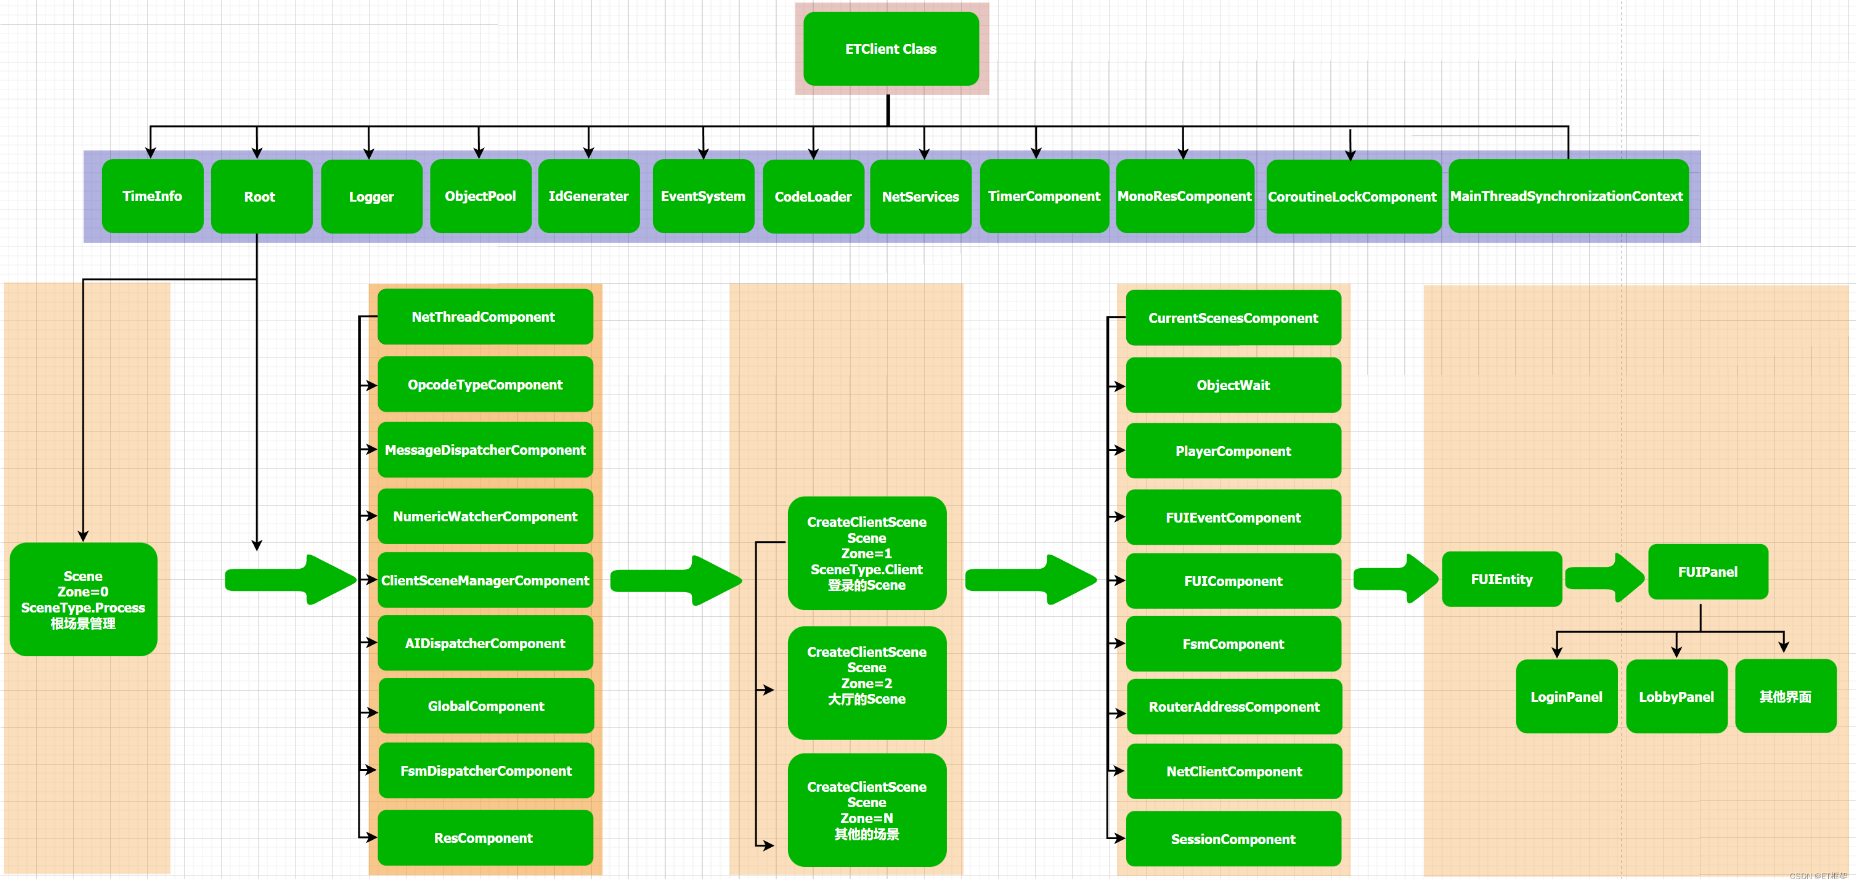
\includegraphics[width=.9\linewidth]{./pic/ET_20230512_143227.png}
\begin{itemize}
\item 【任何时候,活宝妹就是一定要嫁给亲爱的表哥!!!】
\item 【活宝妹坐等亲爱的表哥,领娶活宝妹回家!爱表哥,爱生活!!!】
\end{itemize}
% Emacs 28.2 (Org mode 8.2.7c)
\end{document}